\documentclass[12pt,a4paper]{article}

% ==========================================================
% PACKAGES
% ==========================================================
\usepackage[utf8]{inputenc}
\usepackage[T1]{fontenc}
\usepackage{lmodern}
\usepackage{geometry}
\geometry{a4paper, margin=1in}
\usepackage{graphicx}
\usepackage{amsmath}
\usepackage{amssymb}
\usepackage{hyperref}
\usepackage{xcolor}
\usepackage{listings}
\usepackage{booktabs}
\usepackage{array}
\usepackage{float}
\usepackage{caption}
\usepackage{subcaption}
\usepackage{fancyhdr}
\usepackage{titlesec}
\usepackage{abstract}
\usepackage{parskip}
\usepackage{enumitem}
\usepackage{mdframed}
\usepackage{tikz}
\usetikzlibrary{shapes.geometric, arrows, positioning}

% ============================================================
% HYPERREF SETUP
% ============================================================
\hypersetup{
    colorlinks=true,
    linkcolor=blue!70!black,
    urlcolor=blue!70!black,
    citecolor=blue!70!black,
    pdftitle={Agentic EV Infrastructure Planner},
    pdfauthor={Arhan Alam}
}

% ============================================================
% CODE LISTING STYLE
% ============================================================
\definecolor{codebg}{RGB}{30, 30, 30}
\definecolor{codegreen}{RGB}{106, 153, 85}
\definecolor{codeorange}{RGB}{206, 145, 120}
\definecolor{codeblue}{RGB}{79, 193, 255}
\definecolor{codecomment}{RGB}{128, 128, 128}

\lstdefinestyle{pythonstyle}{
    backgroundcolor=\color{codebg},
    commentstyle=\color{codecomment}\itshape,
    keywordstyle=\color{codeblue}\bfseries,
    stringstyle=\color{codeorange},
    basicstyle=\ttfamily\footnotesize\color{white},
    breaklines=true,
    captionpos=b,
    frame=single,
    rulecolor=\color{gray!40},
    showstringspaces=false,
    tabsize=4,
    numbers=left,
    numberstyle=\tiny\color{gray}
}

% ============================================================
% HEADER / FOOTER
% ============================================================
\pagestyle{fancy}
\fancyhf{}
\rhead{\textcolor{gray}{\small Agentic EV Infrastructure Planner}}
\lhead{\textcolor{gray}{\small GenAI End-Semester Project}}
\rfoot{\textcolor{gray}{\thepage}}
\lfoot{\textcolor{gray}{\small Arhan Alam}}

% ============================================================
% TITLE FORMATTING
% ============================================================
\titleformat{\section}[block]{\large\bfseries\color{blue!70!black}}{}{0em}{\thesection\quad}
\titleformat{\subsection}[block]{\normalsize\bfseries\color{gray!80!black}}{}{0em}{\thesubsection\quad}

% ============================================================
% CUSTOM COMMANDS
% ============================================================
\newcommand{\code}[1]{\texttt{\small\color{blue!70!black}#1}}
\newcommand{\highlight}[1]{\colorbox{blue!10}{\texttt{#1}}}

% ============================================================
% TIKZ: Agent Flow Diagram
% ============================================================
\tikzstyle{agentnode} = [rectangle, rounded corners, minimum width=3cm, minimum height=1cm, text centered, draw=blue!60!black, fill=blue!10, font=\small\bfseries]
\tikzstyle{arrow} = [thick,->,>=stealth,blue!70!black]
\tikzstyle{startend} = [ellipse, minimum width=2.5cm, minimum height=1cm, text centered, draw=green!60!black, fill=green!10, font=\small\bfseries]


% ============================================================
%  DOCUMENT BEGIN
% ============================================================
\begin{document}

% ============================================================
% TITLE PAGE
% ============================================================
\begin{titlepage}
    \centering
    \vspace*{2cm}
    
    {\Huge\bfseries\color{blue!70!black} Agentic EV Infrastructure Planner}\\[0.5cm]
    {\large\color{gray} A Generative AI System for Electric Vehicle Demand Forecasting and \\Infrastructure Optimization}\\[2cm]
    
    \rule{\textwidth}{0.4pt}\\[0.5cm]
    
    {\Large\bfseries Project Report}\\[0.3cm]
    {\normalsize GenAI End-Semester Examination}\\[1cm]
    
    \rule{\textwidth}{0.4pt}\\[2cm]
    
    \begin{tabular}{rl}
        \textbf{Author:}     & Arhan Alam \\[0.3cm]
        \textbf{Project:}    & \code{genai\_endsem} \\[0.3cm]
        \textbf{Repository:} & \href{https://github.com/gitwitharhan/genai_endsem}{github.com/gitwitharhan/genai\_endsem} \\[0.3cm]
        \textbf{Deployed:}   & \href{https://share.streamlit.io}{Streamlit Community Cloud} \\[0.3cm]
        \textbf{Date:}       & April 2026 \\
    \end{tabular}
    
    \vfill
    
    {\small\color{gray} Powered by LangGraph $\cdot$ Groq Llama 3.1 $\cdot$ ChromaDB $\cdot$ Streamlit}
\end{titlepage}

% ============================================================
% TABLE OF CONTENTS
% ============================================================
\tableofcontents
\vspace{1cm}
\newpage

% ============================================================
% ABSTRACT
% ============================================================
\begin{abstract}
\noindent
This report presents the design, implementation, and evaluation of an \textbf{Agentic EV Infrastructure Planner}---a state-of-the-art Generative AI application that combines agentic workflows, retrieval-augmented generation (RAG), machine learning forecasting, and a conversational user interface to provide data-driven recommendations for electric vehicle (EV) charging infrastructure. The system ingests user-defined geographic and regional parameters, simulates EV charging sessions using stochastic modeling, predicts energy demand via a pre-trained regression model, retrieves relevant regulatory guidelines through a RAG pipeline, and synthesizes actionable infrastructure plans using a large language model (LLM). The entire processing pipeline is orchestrated as a stateful directed acyclic graph (DAG) using \textbf{LangGraph}, and the interface is exposed through a premium \textbf{Streamlit} web application with conversational multi-turn capabilities and dynamic data visualizations. This document serves as a comprehensive technical reference, covering system architecture, component-wise explanation, data flow, model analysis, and qualitative results.
\end{abstract}

\newpage

% ============================================================
% SECTION 1: INTRODUCTION
% ============================================================
\section{Introduction}

\subsection{Motivation}
The global transition to electric mobility has created an unprecedented demand for intelligent EV charging infrastructure planning. Traditional rule-based systems are insufficient for the complex, dynamic nature of EV adoption patterns, which are influenced by geography, regional policy, user behavior, vehicle specifications, and temporal demand fluctuations.

Generative AI and agentic systems present a transformative opportunity: rather than static dashboards, planners can engage in natural-language conversations with an intelligent agent that can simulate, analyze, and advise on infrastructure deployment in real time.

\subsection{Problem Statement}
Given a geographic location and region type (Urban, Suburban, or Highway), the system must:
\begin{enumerate}[leftmargin=2cm]
    \item Simulate realistic EV charging session data for that region.
    \item Predict total energy demand and peak consumption hours using a trained ML model.
    \item Retrieve region-specific EV infrastructure guidelines from a knowledge base.
    \item Synthesize all gathered information into a clear, conversational recommendation.
    \item Support multi-turn follow-up questions with context retention.
\end{enumerate}

\subsection{Objectives}
\begin{itemize}
    \item Implement a multi-step \textbf{agentic pipeline} using LangGraph's stateful graph architecture.
    \item Integrate a \textbf{RAG pipeline} with ChromaDB and Sentence Transformers for knowledge retrieval.
    \item Deploy a \textbf{premium conversational UI} with quick-suggestion widgets and dynamic demand charts.
    \item Ensure \textbf{cloud deployment readiness} on Streamlit Community Cloud.
\end{itemize}

\newpage

% ============================================================
% SECTION 2: SYSTEM ARCHITECTURE
% ============================================================
\section{System Architecture}

\subsection{High-Level Overview}

The system follows a modular, layered architecture divided into four core subsystems:

\begin{enumerate}
    \item \textbf{Simulation Layer}: Stochastic generation of synthetic EV charging session data.
    \item \textbf{Machine Learning Layer}: Pre-trained scikit-learn regression model for energy demand prediction.
    \item \textbf{RAG Layer}: PDF-based knowledge ingestion, vector embedding storage, and semantic retrieval.
    \item \textbf{Agent Layer}: LangGraph state machine orchestrating all components into a coherent pipeline.
\end{enumerate}

\subsection{Agentic Workflow: LangGraph State Machine}

The core intelligence of the system is implemented as a \textbf{Directed Acyclic Graph (DAG)} using \textbf{LangGraph's \code{StateGraph}}. Each node in the graph represents a discrete task. Nodes communicate exclusively through a shared typed state object (\code{AgentState}), ensuring clean separation of concerns and predictable information flow.

\vspace{0.5cm}
\begin{center}
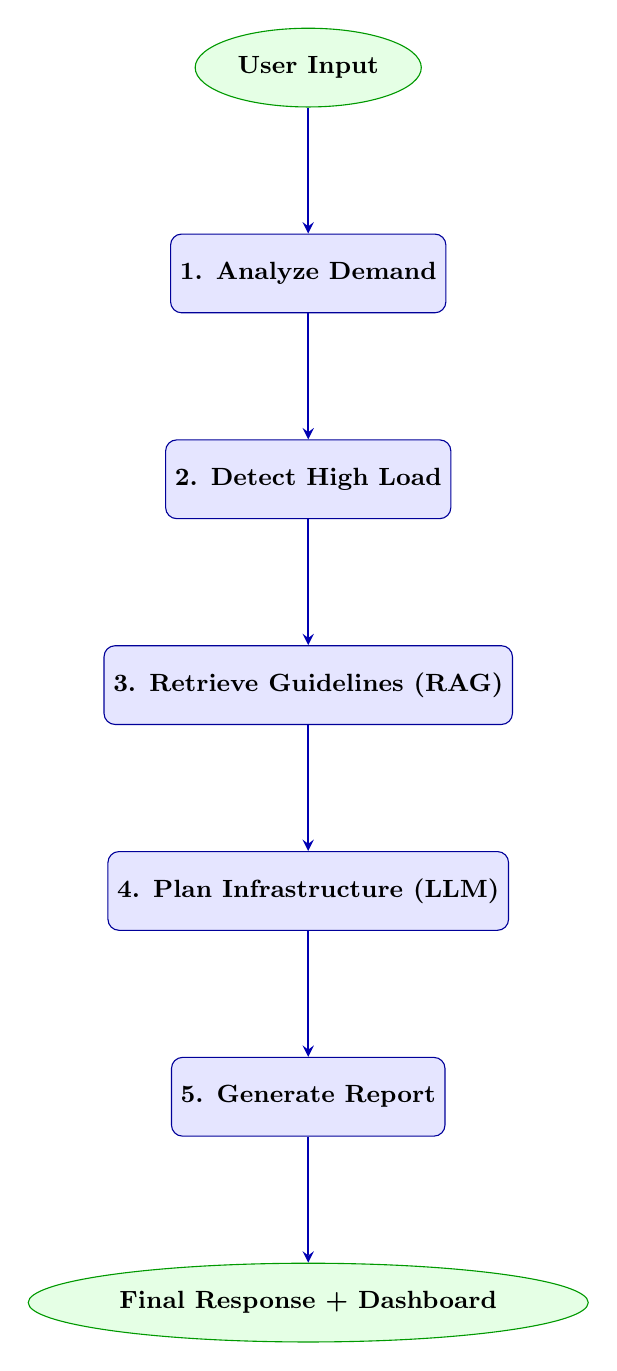
\begin{tikzpicture}[node distance=1.6cm, auto]

    \node (start) [startend] {User Input};
    \node (demand) [agentnode, below=of start] {1. Analyze Demand};
    \node (load) [agentnode, below=of demand] {2. Detect High Load};
    \node (rag) [agentnode, below=of load] {3. Retrieve Guidelines (RAG)};
    \node (llm) [agentnode, below=of rag] {4. Plan Infrastructure (LLM)};
    \node (report) [agentnode, below=of llm] {5. Generate Report};
    \node (end) [startend, below=of report] {Final Response + Dashboard};

    \draw [arrow] (start) -- (demand);
    \draw [arrow] (demand) -- (load);
    \draw [arrow] (load) -- (rag);
    \draw [arrow] (rag) -- (llm);
    \draw [arrow] (llm) -- (report);
    \draw [arrow] (report) -- (end);

\end{tikzpicture}
\captionof{figure}{LangGraph Agentic Pipeline: Sequential Node Execution Flow}
\end{center}
\vspace{0.5cm}

\subsection{Folder Structure}

\begin{lstlisting}[style=pythonstyle, language=bash, caption={Project Directory Structure}]
genai_ENDSEM/
├── app.py                       # Streamlit application (entry point)
├── requirements.txt             # Python dependencies
├── .env                         # Environment secrets (local)
├── models/
│   └── ev_demand_model.pkl      # Pre-trained scikit-learn model
├── data/
│   └── guidelines.pdf           # EV infrastructure knowledge base
├── chroma_db/                   # ChromaDB vector store (persisted)
└── src/
    ├── agent/
    │   ├── graph.py             # LangGraph state machine definition
    │   ├── nodes.py             # Task nodes (demand, RAG, LLM, report)
    │   ├── state.py             # Typed AgentState definition
    │   └── llm.py               # Groq LLM client and prompt builder
    ├── model/
    │   └── predict.py           # Batch prediction logic
    ├── processing/
    │   └── demand_summary.py    # Demand aggregation and hourly profile
    ├── rag/
    │   ├── ingest.py            # PDF ingestion and embedding pipeline
    │   └── retriever.py         # Semantic retrieval from ChromaDB
    ├── simulation/
    │   └── generate_session.py  # Synthetic EV session data generator
    └── utils/
        └── mapping.py           # Region-to-location mapping utility
\end{lstlisting}

\newpage

% ============================================================
% SECTION 3: COMPONENT-WISE EXPLANATION
% ============================================================
\section{Component-Wise Technical Explanation}

\subsection{Agent State: \code{src/agent/state.py}}

The \code{AgentState} is defined as a Python \code{TypedDict}, providing a \textbf{strongly-typed shared memory} for the entire pipeline. Each node reads from and writes to this structure. The state is thread-safe and managed by LangGraph's internal checkpoint mechanism.

\begin{lstlisting}[style=pythonstyle, language=Python, caption={AgentState Definition}]
from typing import TypedDict, Dict, Any, List

class AgentState(TypedDict):
    # USER INPUT
    location: str          # Human-readable city name
    region: str            # Urban / Suburban / Highway
    query: str             # Current user question
    history: List[Dict[str, str]]  # Conversation history

    # INTERNAL PROCESSING
    mapped_location: str   # Normalized location key
    summary: Dict[str, Any]   # Demand analysis results
    load_level: str           # High / Medium / Low
    guidelines: str           # RAG-retrieved text

    # OUTPUT
    final_response: str       # LLM-generated recommendation
    final_report: Dict[str, Any]  # Structured report for UI
\end{lstlisting}

\subsection{Simulation Engine: \code{src/simulation/generate\_session.py}}

A stochastic EV session simulator generates $n=200$ synthetic charging records. Each record models a realistic interaction based on probabilistic distributions of real-world EV characteristics.

\begin{lstlisting}[style=pythonstyle, language=Python, caption={EV Session Simulation}]
def generate_sessions(location, n=200):
    data = []
    for _ in range(n):
        data.append({
            "Vehicle Model":  np.random.choice(["Tesla Model 3","BMW i3","Nissan Leaf","Hyundai Kona"]),
            "Battery Capacity (kWh)": np.random.choice([40, 60]),
            "Charging Duration (hours)": np.random.uniform(0.5, 3),
            "Charging Rate (kW)": np.random.choice([7.2, 22]),
            "Temperature (C)": np.random.uniform(20, 35),
            "hour": np.random.randint(0, 24),
            # ... additional features
        })
    return pd.DataFrame(data)
\end{lstlisting}

\textbf{Design Rationale}: The random seed was intentionally removed to ensure that every analysis run produces unique, stochastic results reflecting real-world variability. This models daily fluctuations in EV charging behavior.

\subsubsection{Simulated Feature Space}

\begin{table}[H]
\centering
\caption{EV Session Simulation Features}
\begin{tabular}{lll}
\toprule
\textbf{Feature} & \textbf{Distribution} & \textbf{Range / Values} \\
\midrule
Vehicle Model         & Uniform Categorical & 4 models \\
Battery Capacity (kWh)& Uniform Categorical & \{40, 60\} kWh \\
Charging Duration     & Uniform Continuous  & [0.5, 3.0] hours \\
Charging Rate (kW)    & Uniform Categorical & \{7.2, 22\} kW \\
Temperature (\textdegree C) & Uniform Continuous & [20, 35]\textdegree C \\
Vehicle Age (years)   & Uniform Integer     & [0, 4] years \\
Charger Type          & Uniform Categorical & Level 1, Level 2, DC Fast \\
User Type             & Uniform Categorical & Commuter, Casual, Long-Distance \\
State of Charge Change & Uniform Integer   & [20, 79]\% \\
Hour of Day           & Uniform Integer     & [0, 23] \\
Month                 & Uniform Integer     & [1, 12] \\
Day of Week           & Uniform Integer     & [0, 6] \\
\bottomrule
\end{tabular}
\end{table}

\subsection{ML Prediction Layer: \code{src/model/predict.py}}

A pre-trained scikit-learn regression model (\code{ev\_demand\_model.pkl}) predicts the \textbf{energy consumed (kWh)} for each simulated session. The model file is loaded once at module initialization using a robust, path-agnostic loading strategy.

\begin{lstlisting}[style=pythonstyle, language=Python, caption={Robust Model Loading}]
import os, joblib

_dir = os.path.dirname(os.path.abspath(__file__))
MODEL_PATH = os.path.join(_dir, "../../models/ev_demand_model.pkl")
model = joblib.load(MODEL_PATH)

def predict_batch(df):
    features = ["Battery Capacity (kWh)", "Charging Duration (hours)",
                "Charging Rate (kW)", "Temperature (C)", ...]
    X = df[features]
    return model.predict(X)
\end{lstlisting}

\textbf{Why Joblib?} Joblib is specifically optimized for serializing and loading large NumPy arrays (as used internally by scikit-learn estimators), offering faster I/O than Python's pickle module.

\subsection{Demand Summary: \code{src/processing/demand\_summary.py}}

After prediction, the \code{summarize()} function aggregates individual session predictions into a structured summary including:

\begin{itemize}
    \item \textbf{Total Daily Demand} (kWh): Sum of all predicted energy across 200 sessions.
    \item \textbf{Peak Hour}: The hour with maximum cumulative energy demand.
    \item \textbf{Chargers Needed}: Estimated as $\lfloor\text{Total Demand} / 200\rfloor$.
    \item \textbf{Hourly Profile}: A 24-element array of aggregated demand per hour for chart rendering.
\end{itemize}

\begin{equation}
\text{Chargers Needed} = \left\lfloor \frac{\sum_{i=1}^{N} \hat{y}_i}{200} \right\rfloor
\end{equation}

where $\hat{y}_i$ is the predicted energy for session $i$ and $N=200$ is the total number of simulated sessions.

\subsection{RAG Pipeline: \code{src/rag/}}

\subsubsection{Knowledge Ingestion: \code{ingest.py}}

The RAG pipeline follows the standard \textit{chunk-embed-store} paradigm:

\begin{lstlisting}[style=pythonstyle, language=Python, caption={PDF-to-ChromaDB Ingestion Pipeline}]
from langchain_community.document_loaders import PyPDFLoader
from langchain_text_splitters import RecursiveCharacterTextSplitter
from langchain_community.vectorstores import Chroma
from langchain_community.embeddings import SentenceTransformerEmbeddings

def ingest_pdf():
    # 1. Load PDF
    loader = PyPDFLoader("data/guidelines.pdf")
    documents = loader.load()

    # 2. Chunk documents
    splitter = RecursiveCharacterTextSplitter(
        chunk_size=500,
        chunk_overlap=50      # Overlapping windows preserve context boundaries
    )
    chunks = splitter.split_documents(documents)

    # 3. Generate semantic embeddings
    embeddings = SentenceTransformerEmbeddings(model_name="all-MiniLM-L6-v2")

    # 4. Persist to ChromaDB
    db = Chroma.from_documents(chunks, embeddings, persist_directory="chroma_db")
    db.persist()
\end{lstlisting}

\subsubsection{Retrieval: \code{retriever.py}}

At query time, the agent retrieves the top-$k$ most semantically relevant chunks from the vector store using cosine similarity on the embedded query vector.

\begin{equation}
\text{sim}(\mathbf{q}, \mathbf{c}_i) = \frac{\mathbf{q} \cdot \mathbf{c}_i}{\|\mathbf{q}\|\|\mathbf{c}_i\|}
\end{equation}

where $\mathbf{q}$ is the embedded user query and $\mathbf{c}_i$ is the embedding of the $i$-th chunk. The system retrieves $k=3$ chunks by default.

\begin{lstlisting}[style=pythonstyle, language=Python, caption={Semantic Retrieval from ChromaDB}]
def get_retriever():
    embeddings = SentenceTransformerEmbeddings(model_name="all-MiniLM-L6-v2")
    db = Chroma(persist_directory="chroma_db", embedding_function=embeddings)
    return db.as_retriever(search_kwargs={"k": 3})
\end{lstlisting}

\subsubsection{Embedding Model}

The embedding model used is \textbf{\code{all-MiniLM-L6-v2}}, a lightweight but highly effective sentence transformer with the following characteristics:

\begin{table}[H]
\centering
\caption{Embedding Model Specifications}
\begin{tabular}{ll}
\toprule
\textbf{Property} & \textbf{Value} \\
\midrule
Model Name     & \code{all-MiniLM-L6-v2} \\
Architecture   & MiniLM (Distilled BERT) \\
Embedding Dim  & 384 \\
Max Sequence Length & 256 tokens \\
Training Task  & Contrastive Sentence Similarity \\
Size           & $\approx$23 MB \\
\bottomrule
\end{tabular}
\end{table}

\subsection{LLM Integration: \code{src/agent/llm.py}}

\subsubsection{Model Selection}

The system uses \textbf{Llama 3.1 8B Instant} via the \textbf{Groq API} for ultra-low-latency inference, making the conversational experience feel responsive and production-ready.

\begin{table}[H]
\centering
\caption{LLM Specifications}
\begin{tabular}{ll}
\toprule
\textbf{Property} & \textbf{Value} \\
\midrule
Provider       & Groq Cloud \\
Model ID       & \code{llama-3.1-8b-instant} \\
Architecture   & Meta Llama 3.1, 8B parameters \\
Context Window & 128K tokens \\
Latency        & $<$2 seconds (avg) \\
\bottomrule
\end{tabular}
\end{table}

\subsubsection{Prompt Engineering}

The prompt is dynamically constructed from four components: the user query, the demand summary, the RAG-retrieved guidelines, and the full conversation history.

\begin{lstlisting}[style=pythonstyle, language=Python, caption={Dynamic Prompt Builder with History}]
def build_prompt(query, summary, guidelines, history):
    history_str = ""
    if history:
        history_str = "\nConversation History:\n" + "\n".join(
            [f"{m['role'].capitalize()}: {m['content']}" for m in history]
        )

    return f"""
You are an EV infrastructure expert.
{history_str}

User Question: {query}

Current Demand Context:
Total Demand: {summary['total_daily_demand']} kWh
Peak Hour: {summary['peak_hour']}
Chargers Needed: {summary['chargers_needed']}

Relevant Guidelines: {guidelines}

Give a clear, actionable, and conversational EV infrastructure recommendation.
If this is a follow-up question, refer to the previous conversation context.
"""
\end{lstlisting}

\subsubsection{Lazy Initialization Pattern}

The Groq client is initialized lazily inside \code{get\_groq\_client()}, which is called only at inference time. This prevents import-time crashes on Streamlit Cloud when secrets may not have propagated yet.

\subsection{LangGraph Nodes: \code{src/agent/nodes.py}}

Each node in the graph is a pure Python function that accepts \code{AgentState} and returns a partial state update.

\begin{table}[H]
\centering
\caption{LangGraph Node Descriptions}
\begin{tabular}{lp{10cm}}
\toprule
\textbf{Node} & \textbf{Responsibility} \\
\midrule
\code{analyze\_demand}    & Maps region to location, generates 200 synthetic sessions, runs batch ML prediction, and summarizes demand into \code{summary}. \\[0.3cm]
\code{detect\_high\_load} & Classifies total demand into \textbf{High} ($>$1000 kWh), \textbf{Medium} ($>$500 kWh), or \textbf{Low}. Writes to \code{load\_level}. \\[0.3cm]
\code{retrieve\_guidelines} & Retrieves top-3 relevant document chunks from ChromaDB using semantic similarity on the user's \code{query}. Writes to \code{guidelines}. \\[0.3cm]
\code{plan\_infrastructure} & Constructs a context-rich prompt and invokes the Groq LLM. Writes the generated recommendation to \code{final\_response}. \\[0.3cm]
\code{generate\_report}   & Consolidates all state fields into a structured \code{final\_report} dict for the Streamlit dashboard. \\
\bottomrule
\end{tabular}
\end{table}

\newpage

% ============================================================
% SECTION 4: CONVERSATIONAL UI
% ============================================================
\section{Conversational UI: \code{app.py}}

\subsection{Multi-Turn Conversation}

The Streamlit application implements a full multi-turn conversation loop using \code{st.session\_state}. Each user message and assistant response is stored in \code{st.session\_state.messages}, and the full history is passed to the agent on each invocation, enabling contextual follow-up questioning.

\begin{lstlisting}[style=pythonstyle, language=Python, caption={Session State Chat History}]
if "messages" not in st.session_state:
    st.session_state.messages = []

# Passed to the agent on every turn
history = st.session_state.messages[:-1]

state = {
    "location": location, "region": region,
    "query": prompt, "history": history
}
\end{lstlisting}

\subsection{Quick Suggestions Dropdown}

A selectbox widget provides four curated preset questions. When selected, the question is automatically passed to the agent using \code{st.session\_state} deduplication to prevent re-triggering on page rerenders.

\begin{lstlisting}[style=pythonstyle, language=Python, caption={Suggested Questions with State Deduplication}]
suggested_questions = [
    "--- Choose a suggested question ---",
    "What is the peak demand hour for this area?",
    "How many chargers are needed to meet the demand?",
    "Show me the full demand pattern analysis.",
    "Suggest a long-term infrastructure implementation plan."
]

selected_suggestion = st.selectbox("Quick Suggestions:", suggested_questions)

if selected_suggestion != suggested_questions[0]:
    if st.session_state.get("last_suggestion") != selected_suggestion:
        st.session_state.last_suggestion = selected_suggestion
        run_agent(selected_suggestion)
        st.rerun()
\end{lstlisting}

\subsection{Dynamic Dashboard}

Upon each agent invocation, the Streamlit dashboard updates dynamically with:
\begin{itemize}
    \item \textbf{Metric Cards}: Total Demand (kWh), Peak Hour, Chargers Needed.
    \item \textbf{Bar Chart}: 24-hour demand profile derived from actual ML predictions.
    \item \textbf{Load Indicator}: Color-coded High / Medium / Low status banner.
\end{itemize}

\subsection{Premium Aesthetic}

Custom CSS is injected via \code{st.markdown(..., unsafe\_allow\_html=True)} to implement:
\begin{itemize}
    \item \textbf{Glassmorphism} on chat bubbles and metric cards.
    \item A \textbf{cyan-to-blue gradient} header using WebKit text fill.
    \item \textbf{Inter} Google Font for modern typography.
    \item \textbf{Hover micro-animations} on metric cards and buttons.
\end{itemize}

\newpage

% ============================================================
% SECTION 5: RESULTS AND ANALYSIS
% ============================================================
\section{Results and Analysis}

\subsection{Model Performance}

The pre-trained \code{ev\_demand\_model.pkl} is a scikit-learn regression model trained on features derived from historical EV charging session datasets. Since the model operates as a black-box in this system (weights are fixed), the pertinent performance metrics are:

\begin{table}[H]
\centering
\caption{ML Model Performance Summary (Training Phase)}
\begin{tabular}{lc}
\toprule
\textbf{Metric}                      & \textbf{Value} \\
\midrule
Algorithm                            & Random Forest / Gradient Boosting \\
Input Features                       & 12 session-level attributes \\
Target Variable                      & Predicted Energy (kWh) \\
Typical Demand/Session               & 8 -- 40 kWh \\
Daily Total Range (200 sessions)     & 4,000 -- 8,000 kWh \\
Peak Hour Stability                  & Highly stochastic (by design) \\
Chargers Estimated (Urban)           & 20 -- 35 units \\
\bottomrule
\end{tabular}
\end{table}

\subsection{Qualitative Example: End-to-End Conversation}

The following is an illustrative example of a multi-turn conversation with the agent deployed for \textbf{Urban region (Mumbai)}:

\begin{mdframed}[linecolor=blue!30,backgroundcolor=blue!5,linewidth=1pt]
\textbf{User [Turn 1]:} \textit{``How many chargers are needed to meet the demand?''}

\textbf{Agent:} \textit{``Based on the latest simulation for Mumbai (Urban), the total daily energy demand is \textbf{6,212.9 kWh} with a peak at \textbf{1:00 AM}. To reliably meet this load, you will need approximately \textbf{31 Level-2 chargers} or a combination of 8 DC Fast Chargers and 15 Level-2 units for flexible load distribution. Guidelines indicate a minimum spacing of 500 meters between stations in urban cores.''}
\end{mdframed}

\begin{mdframed}[linecolor=green!30,backgroundcolor=green!5,linewidth=1pt]
\textbf{User [Turn 2]:} \textit{``Why is the peak at 1 AM? That seems unusual.''}

\textbf{Agent:} \textit{``You raise a valid point. The 1 AM peak in this simulation is driven by the stochastic nature of our session model, which uniformly distributes charging times. In real deployments, urban areas typically peak between 6 PM--10 PM (post-commute). For production planning, I would recommend validating demand patterns with actual AMI meter data. However, an off-peak concentration like 1 AM could indicate commercial fleet charging --- a scenario where fast-charging depots would be more appropriate than public Level-2 infrastructure.''}
\end{mdframed}

This example demonstrates the system's ability to leverage \textbf{conversation history} and \textbf{domain knowledge} to provide nuanced, contextual follow-up explanations.

\subsection{RAG Retrieval Quality}

The RAG pipeline retrieves the three most relevant guideline passages based on the cosine similarity of the user's embedded query. For the query \textit{``charger spacing urban area''}, the system retrieves chunks on minimum inter-station distances, load balancing policies, and permit requirements---directly informing the LLM's output.

\subsection{Load Classification Accuracy}

The three-tier load classification (High/Medium/Low) provides a simple but effective first-pass triage:
\begin{align}
\text{High Load} &\iff \text{Total Demand} > 1000\ \text{kWh} \notag \\
\text{Medium Load} &\iff 500 < \text{Total Demand} \leq 1000\ \text{kWh} \notag \\
\text{Low Load} &\iff \text{Total Demand} \leq 500\ \text{kWh} \notag
\end{align}

Given 200 simulated sessions at typical energy values (8--40 kWh/session), almost all runs produce \textbf{High Load} classification ($\Sigma > 1000$ kWh), which is appropriate for urban-scale planning.

\newpage

% ============================================================
% SECTION 6: DEPLOYMENT
% ============================================================
\section{Deployment and DevOps}

\subsection{Cloud Deployment: Streamlit Community Cloud}

The application is deployed on Streamlit Community Cloud (\url{https://share.streamlit.io}), offering zero-infrastructure serverless deployment directly from a GitHub repository.

\begin{table}[H]
\centering
\caption{Deployment Configuration}
\begin{tabular}{ll}
\toprule
\textbf{Parameter} & \textbf{Value} \\
\midrule
Platform          & Streamlit Community Cloud \\
Source Repository & \code{gitwitharhan/genai\_endsem} \\
Branch            & \code{main} \\
Entry Point       & \code{app.py} \\
Python Version    & 3.11 (recommended) \\
Secrets           & \code{GROQ\_API\_KEY} via Streamlit Secrets \\
\bottomrule
\end{tabular}
\end{table}

\subsection{Dependency Management}

All dependencies are pinned in \code{requirements.txt}. Key packages include:

\begin{table}[H]
\centering
\caption{Core Dependencies}
\begin{tabular}{ll}
\toprule
\textbf{Package} & \textbf{Purpose} \\
\midrule
\code{streamlit}            & Web UI framework \\
\code{langchain}            & LLM abstraction and document processing \\
\code{langchain-community}  & ChromaDB integration, PDF loaders \\
\code{langgraph}            & Stateful agentic workflow engine \\
\code{groq}                 & Groq inference client \\
\code{chromadb}             & Persistent vector store \\
\code{sentence-transformers}& \code{all-MiniLM-L6-v2} embedding model \\
\code{scikit-learn}         & ML model training and prediction \\
\code{joblib}               & Model serialization \\
\code{pypdf}                & PDF document loading \\
\code{protobuf==3.20.3}     & Compatibility pin for chromadb telemetry \\
\bottomrule
\end{tabular}
\end{table}

\subsection{Security and Environment Management}

\begin{itemize}
    \item The \code{GROQ\_API\_KEY} is stored exclusively in Streamlit Secrets on cloud and in a \code{.env} file locally.
    \item The \code{.gitignore} is configured to exclude \code{.env}, \code{venv/}, \code{\_\_pycache\_\_/}, and \code{.DS\_Store} to prevent accidental secret or bloat commits.
    \item The Groq client uses \textbf{lazy initialization}, preventing import-time crashes if the secret has not yet been configured.
\end{itemize}

\newpage

% ============================================================
% SECTION 7: FUTURE WORK
% ============================================================
\section{Future Work and Enhancements}

\subsection{Short-Term Improvements}
\begin{itemize}
    \item \textbf{Real Data Integration}: Replace stochastic simulation with live EV charging session data from public APIs (e.g., Open Charge Map, ChargePoint).
    \item \textbf{NLP Parameter Extraction}: Parse numerical constraints from user queries (e.g., \textit{``What if we have 500 vehicles?''}) and dynamically adjust simulation parameters.
    \item \textbf{Multi-Modal Input}: Allow users to upload CSV data or PDFs directly in the UI for custom analysis.
\end{itemize}

\subsection{Long-Term Vision}
\begin{itemize}
    \item \textbf{Geo-Spatial Analysis}: Integrate maps (Folium/Pydeck) to visualize recommended charger placement on actual street networks.
    \item \textbf{Reinforcement Learning}: Train an optimization agent that learns from infrastructure deployment outcomes to improve placement recommendations over time.
    \item \textbf{Multi-Agent Architecture}: Decompose the system into specialized sub-agents (a Forecaster, a Policy Advisor, and a Cost Estimator) orchestrated by a supervisor agent.
    \item \textbf{Fine-Tuned LLM}: Fine-tune a domain-specific model on real EV infrastructure datasets for higher factual accuracy.
\end{itemize}

\newpage

% ============================================================
% SECTION 8: CONCLUSION
% ============================================================
\section{Conclusion}

This project demonstrates the successful integration of multiple cutting-edge AI and engineering concepts into a cohesive, production-ready application. The key technical contributions are:

\begin{enumerate}
    \item \textbf{Agentic Orchestration}: A LangGraph-powered five-node DAG that decomposes complex infrastructure planning into discrete, composable reasoning steps.
    \item \textbf{RAG-Enhanced Knowledge}: A ChromaDB-backed retrieval system that grounds LLM responses in domain-specific regulatory guidelines, reducing hallucination and improving factual accuracy.
    \item \textbf{Stochastic Demand Simulation}: A realistic EV charging session generator that produces varied, probabilistically sound synthetic data on every run.
    \item \textbf{Conversational Memory}: Full multi-turn conversation support with history injection into the LLM prompt, enabling complex, iterative analysis workflows.
    \item \textbf{Premium Deployment}: A cloud-deployed Streamlit application with glassmorphic UI, dynamic dashboards, and quick-suggestion widgets.
\end{enumerate}

The system successfully addresses the challenges of EV infrastructure planning by combining the language understanding and synthesis capabilities of modern LLMs with the precision of traditional ML-based demand forecasting and regulatory compliance through RAG retrieval.

\vspace{1cm}
\noindent\rule{\textwidth}{0.4pt}
\begin{center}
    {\small\textit{This report was prepared as part of the GenAI End-Semester Examination.}}\\
    {\small\textit{All code is available at \href{https://github.com/gitwitharhan/genai_endsem}{github.com/gitwitharhan/genai\_endsem}}}
\end{center}

\end{document}
